\chapter{Demo - Warehouse Manager 1.0.0}

\section{Startbildschirm}

\begin{figure}[h!]
    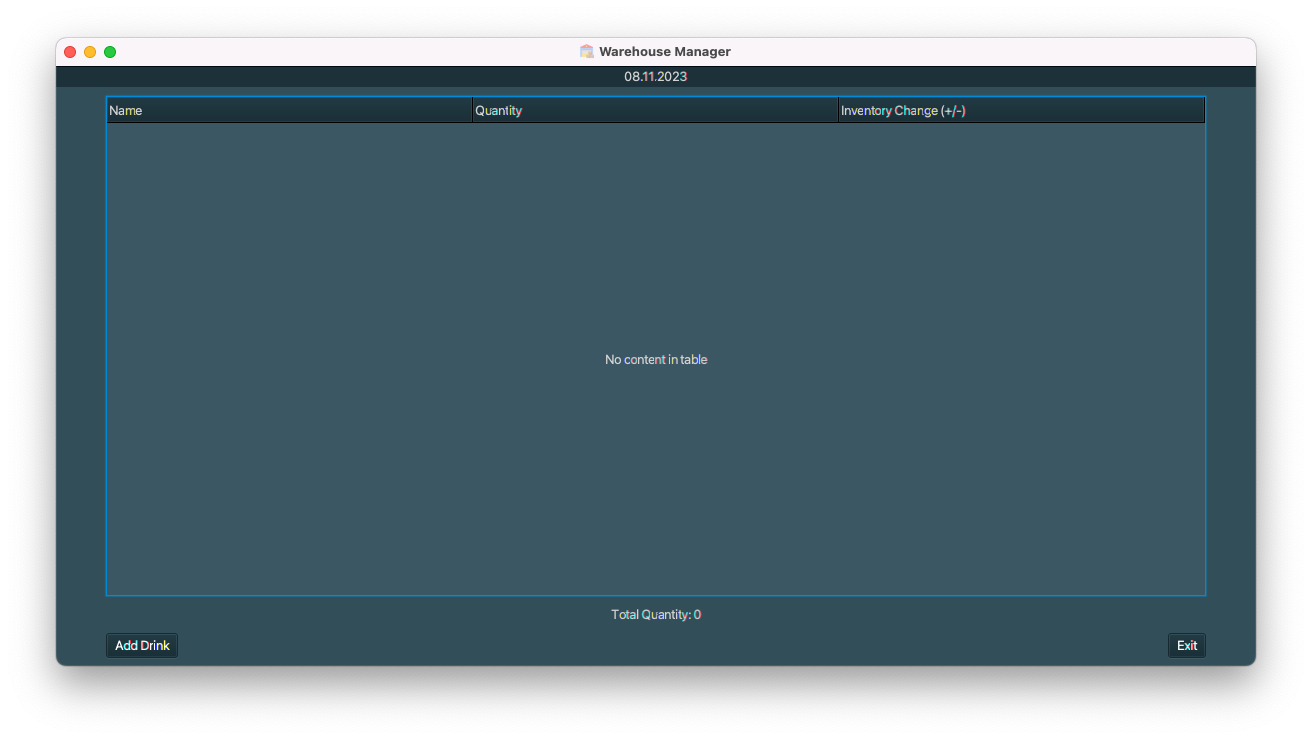
\includegraphics[width=\textwidth]{main_view_empty.png}
    \caption{Startbilschirm wenn keine Getränke vorhanden sind}
    \label{fig:main_view_empty}
\end{figure}

\begin{figure}[h!]
    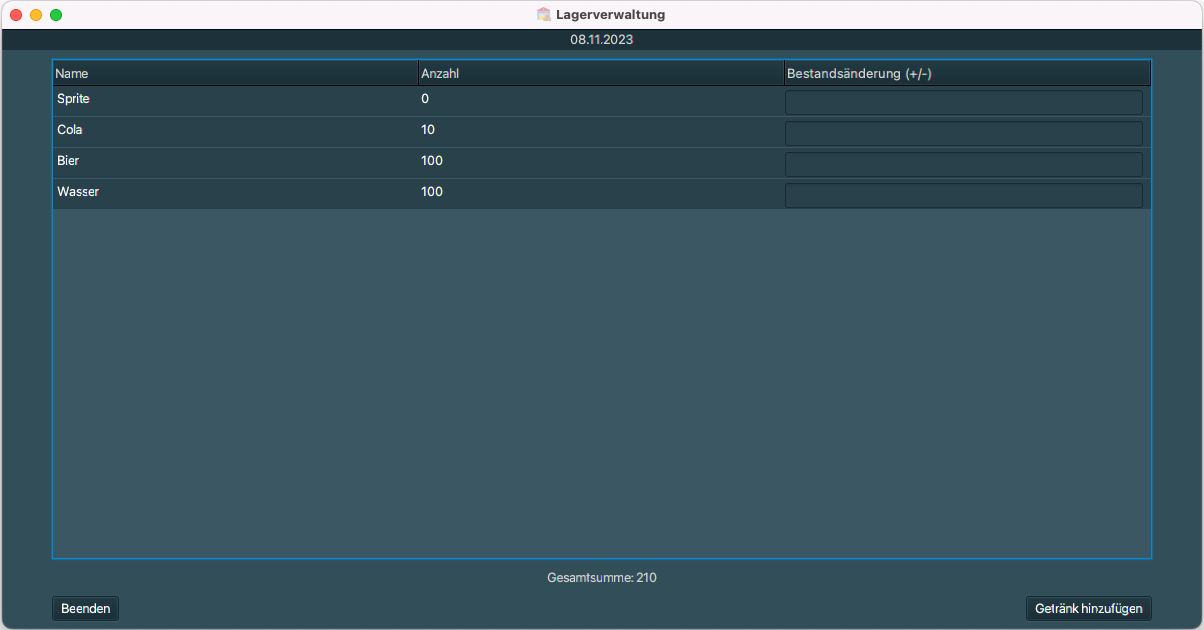
\includegraphics[width=\textwidth]{main_view_filled.png}
    \caption{Startbilschirm wenn Getränke vorhanden sind}
    \label{fig:main_view_filled}
\end{figure}

\clearpage

\section{Getränk hinzufügen}

\begin{figure}[h!]
    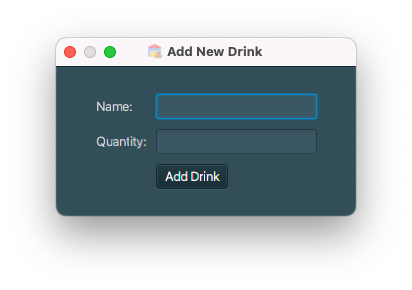
\includegraphics[width=9cm]{add_drink_empty.png}
    \caption{Dialog zum Hinzufügen eines Getränks (leer)}
    \label{fig:add_drink_empty}
\end{figure}

\begin{figure}[h!]
    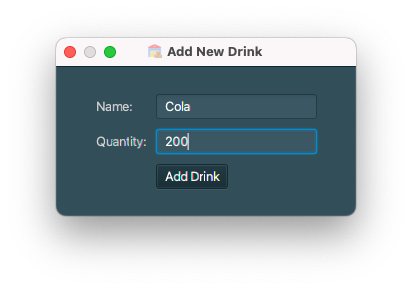
\includegraphics[width=9cm]{add_drink.png}
    \caption{Dialog zum Hinzufügen eines Getränks (ausgefüllt)}
    \label{fig:add_drink}
\end{figure}

\begin{figure}[h!]
    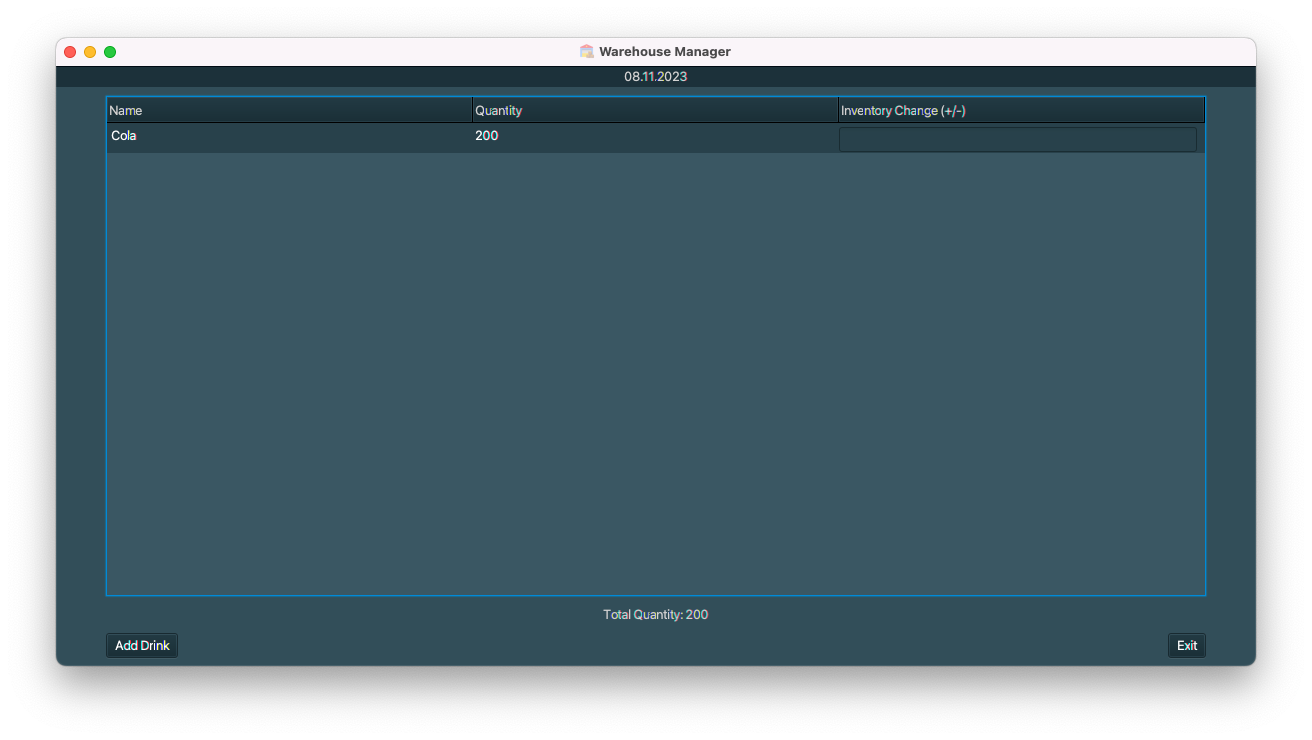
\includegraphics[width=\textwidth]{main_view.png}
    \caption{Startbilschirm nach Hinzufügen eines Getränks}
    \label{fig:main_view}
\end{figure}

\clearpage

\section{Bestandsänderung}


\begin{figure}[h!]
    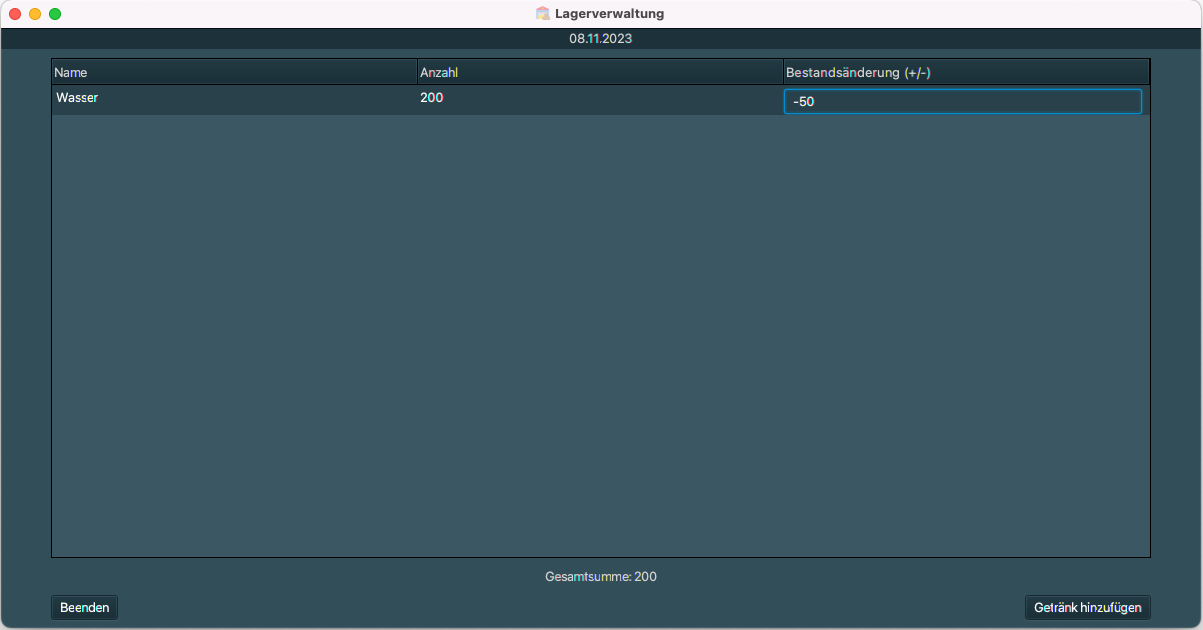
\includegraphics[width=\textwidth]{main_view_change.png}
    \caption{Startbilschirm beim ändern des Bestandes}
    \label{fig:main_view_change}
\end{figure}

\begin{figure}[h!]
    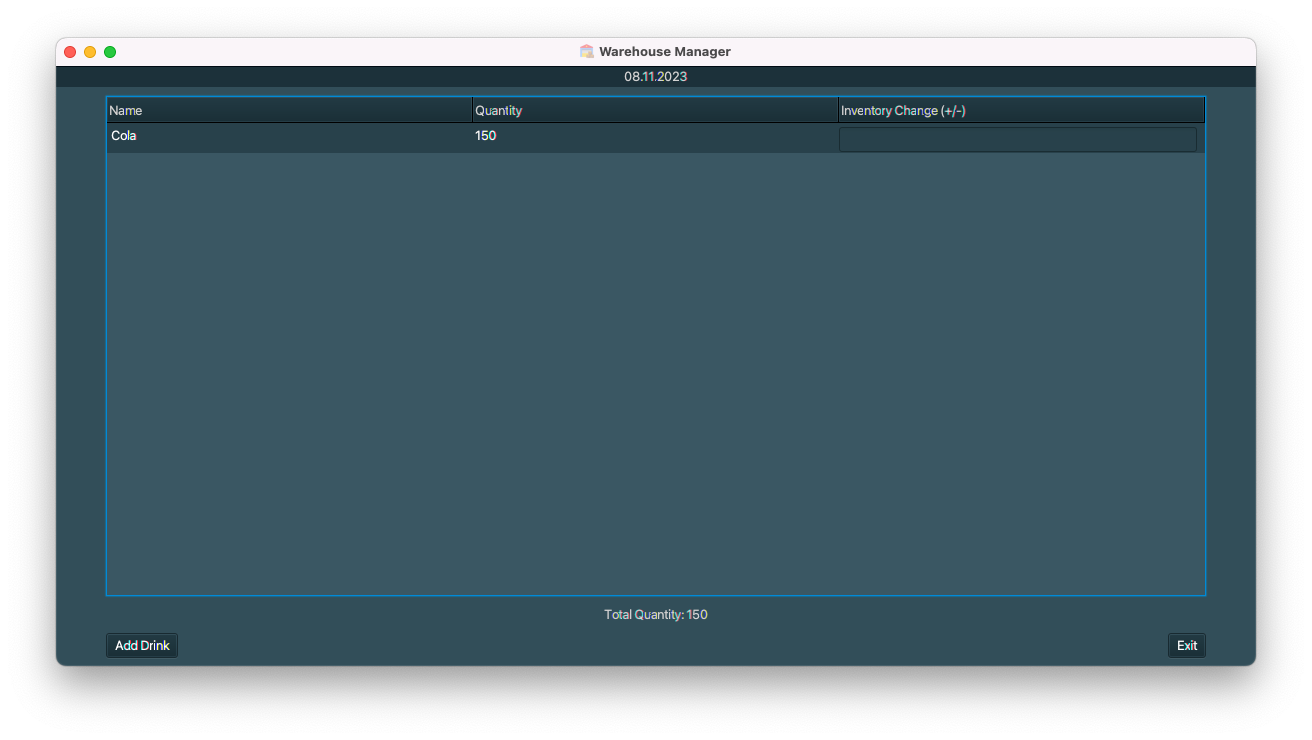
\includegraphics[width=\textwidth]{main_view_change_after.png}
    \caption{Startbilschirm nach dem ändern des Bestandes}
    \label{fig:main_view_change_after}
\end{figure}